\documentclass[fleqn, a4paper, 11pt, oneside]{amsart}
%\usepackage[top = 2cm, bottom = 1cm, left = 1cm, right = 1cm]{geometry}
\usepackage{exsheets, tasks}
\usepackage{amsmath, amssymb, amsthm} %standard AMS packages
\usepackage{marginnote} %marginnotes
\usepackage{gensymb} %miscellaneous symbols
\usepackage{commath} %differential symbols
\usepackage{xcolor} %colours
\usepackage{cancel} %cancelling terms
\usepackage[free-standing-units, space-before-unit]{siunitx} %formatting units
\usepackage{tikz, pgfplots} %diagrams
\usetikzlibrary{calc, hobby, patterns, intersections, decorations.markings}
\usepackage{graphicx} %inserting graphics
\usepackage{hyperref} %hyperlinks
\usepackage{datetime} %date and time
\usepackage{ulem} %underline for \emph{}
\usepackage{xfrac} %inline fractions
\usepackage{enumerate,enumitem} %numbered lists
\usepackage{float} %inserting floats
\usepackage{circuitikz}[american voltages, american currents] %circuit diagrams

\newcommand\numberthis{\addtocounter{equation}{1}\tag{\theequation}} %adds numbers to specific equations in non-numbered list of equations

\newcommand{\AxisRotator}[1][rotate=0]{
	\tikz [x=0.25cm,y=0.60cm,line width=.2ex,-stealth,#1] \draw (0,0) arc (-150:150:1 and 1);%
} %rotation symbols on axes

\theoremstyle{definition}
\newtheorem{example}{Example}
\newtheorem{definition}{Definition}

\theoremstyle{theorem}
\newtheorem{theorem}{Theorem}

\newcommand{\curl}{\mathrm{curl\,}}

\newcommand{\Arg}{\mathrm{Arg}}

\newcommand{\Int}{\mathrm{Int}}
\newcommand{\Ext}{\mathrm{Ext}}
\newcommand{\boundary}{\partial}

\makeatletter
\@addtoreset{section}{part} %resets section numbers in new part
\makeatother

\renewcommand{\thesubsection}{(\arabic{subsection})}
\renewcommand{\thesection}{(\arabic{section})}

%section headings on left
\makeatletter
\def\specialsection{\@startsection{section}{1}%
	\z@{\linespacing\@plus\linespacing}{.5\linespacing}%
	%  {\normalfont\centering}}% DELETED
	{\normalfont}}% NEW
\def\section{\@startsection{section}{1}%
	\z@{.7\linespacing\@plus\linespacing}{.5\linespacing}%
	%  {\normalfont\scshape\centering}}% DELETED
	{\normalfont\scshape}}% NEW
\makeatother

%forces newline after subsection
\makeatletter
\def\subsection{\@startsection{subsection}{3}%
	\z@{.5\linespacing\@plus.7\linespacing}{.1\linespacing}%
	{\normalfont\itshape}}
\makeatother

\settasks{counter-format = tsk[1].}

\SetupExSheets{solution/print = true}

%opening
\title{Complex Functions : Assignment 2}
\author
{
	Aakash Jog\\
	ID : 989323563
}
\date{\formatdate{11}{11}{2015}}

\begin{document}

\tikzset{->-/.style={decoration={
  markings,
  mark=at position #1 with {\arrow{>}}},postaction={decorate}}}

\maketitle
%\setlength{\mathindent}{0pt}

\setcounter{question}{0}
\begin{question}
	Draw the following sets in the complex plane.
	\begin{enumerate}[label=({\alph*})]
		\setcounter{enumi}{5}
		\item $\left\{ z : -1 < \Im(z) < 1 , -1 < \Re(z) < 1 \right\}$
		\setcounter{enumi}{7}
		\item $\left\{ z : |z| < 1 , 0 \le \Arg(z) \le \frac{\pi}{4} \right\}$
	\end{enumerate}
\end{question}

\begin{solution}
	\begin{enumerate}[label=({\alph*}), leftmargin=*]
		\setcounter{enumi}{5}
		\item
			~\\
			\begin{figure}[H]
				\centering
				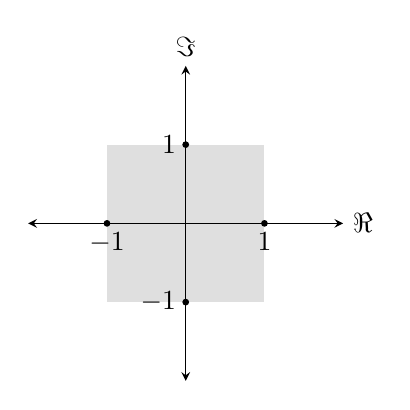
\begin{tikzpicture}
					\def\xMIN{-2};
					\def\xMAX{2};
					\def\yMIN{-2};
					\def\yMAX{2};
	
					\begin{scope}
						\fill [lightgray, opacity = 0.5] (-1,-1) rectangle (1,1);
					\end{scope}

					\begin{scope}[stealth-stealth]
						\draw (\xMIN,0) -- (\xMAX,0) node [right] {$\Re$};
						\draw (0,\yMIN) -- (0,\yMAX) node [above] {$\Im$};
					\end{scope}
	
					\begin{scope}
						\filldraw (-1,0) circle (1pt) node [below] {$-1$};
						\filldraw (1,0) circle (1pt) node [below] {$1$};
	                                         fill
						\filldraw (0,-1) circle (1pt) node [left] {$-1$};
						\filldraw (0,1) circle (1pt) node [left] {$1$};
					\end{scope}
				\end{tikzpicture}
				\caption{$\left\{ z : -1 < \Im(z) < 1 , -1 < \Re(z) < 1 \right\}$}
			\end{figure}
		\setcounter{enumi}{7}
		\item
			~\\
			\begin{figure}[H]
				\centering
				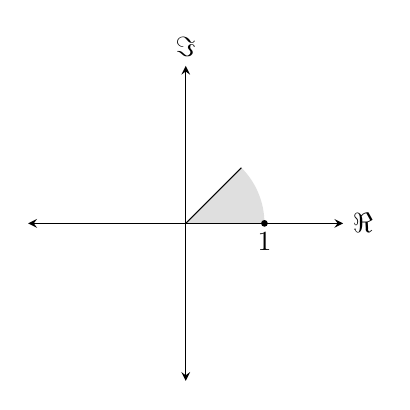
\begin{tikzpicture}
					\def\xMIN{-2};
					\def\xMAX{2};
					\def\yMIN{-2};
					\def\yMAX{2};
	
					\begin{scope}
						\fill [lightgray, opacity = 0.5] (0,0) -- (1,0) arc (0:45:1);
						\draw (0,0) -- ++(0:1);
						\draw (0,0) -- ++(45:1);
					\end{scope}

					\begin{scope}[stealth-stealth]
						\draw (\xMIN,0) -- (\xMAX,0) node [right] {$\Re$};
						\draw (0,\yMIN) -- (0,\yMAX) node [above] {$\Im$};
					\end{scope}
	
					\begin{scope}
						\filldraw (1,0) circle (1pt) node [below] {$1$};
					\end{scope}
				\end{tikzpicture}
			\caption{$\left\{ z : |z| < 1 , 0 \le \Arg(z) \le \frac{\pi}{4} \right\}$}
			\end{figure}
	\end{enumerate}
\end{solution}

\setcounter{question}{2}
\begin{question}
	For every mapping, find where it maps the given set to.
	\begin{enumerate}[label=({\alph*})]
		\setcounter{enumi}{1}
		\item The set $\left\{ z : 0 \le \Arg(z) \le \frac{\pi}{4} \right\}$ under the map $f(z) = z^2$
	\end{enumerate}
\end{question}

\begin{solution}
	\begin{enumerate}[label=({\alph*}), leftmargin=*]
		\setcounter{enumi}{1}
		\item
			Let
			\begin{align*}
				z &= r e^{i \theta}
			\end{align*}
			Therefore,
			\begin{align*}
				z^2 &= r^2 e^{2 i \theta}
			\end{align*}
			Therefore, as $0 \le \theta \le \frac{\pi}{4}$, $0 \le 2 \theta \le \frac{\pi}{2}$.\\
			Therefore, the set $\left\{ z : 0 \le \Arg(z) \le \frac{\pi}{4} \right\}$ maps to $\left\{ z : 0 \le \Arg(z) \le \frac{\pi}{2} \right\}$ under the map $f(z) = z^2$.
	\end{enumerate}
\end{solution}

\setcounter{question}{4}
\begin{question}
	Write the following functions in the form
	\begin{align*}
		f(z) &= u(x,y) + i v(x,y)
	\end{align*}
	Are $u$ and $v$ continuous?
	Where?
	\begin{enumerate}[label=({\alph*})]
		\setcounter{enumi}{2}
		\item $f(z) = z e^{2 z}$
	\end{enumerate}
\end{question}

\begin{solution}
	\begin{enumerate}[label=({\alph*}), leftmargin=*]
		\setcounter{enumi}{2}
		\item
			Let
			\begin{align*}
				z &= x + i y
			\end{align*}
			Therefore,
			\begin{align*}
				f(z) &= z e^{2 z}\\
				&= (x + i y) e^{2 x} e^{2 i y}\\
				&= (x + i y) e^{2 x} \left( \cos(2 y) + i \sin(2 y) \right)\\
				&= e^{2 x} \left( x \cos(2 y) + i x \sin(2 y) + i y \cos(2 y) - y \sin(2 y) \right)\\
				&= e^{2 x} \left( x \cos(2 y) - y \sin(2 y) \right) + i e^{2 x} \left( x \sin(2 y) + y \cos(2 y) \right)
			\end{align*}
			Therefore,
			\begin{align*}
				u(x,y) &= e^{2 x} \left( x \cos(2 y) - y \sin(2 y) \right)\\
				v(x,y) &= e^{2 x} \left( x \sin(2 y) - y \cos(2 y) \right)
			\end{align*}
			$u$ and $v$ are continuous over $\mathbb{R}$.
	\end{enumerate}
\end{solution}

\setcounter{question}{6}
\begin{question}
	Prove, using the differentiability definition only, that $f_1(z) = \Re(z)$ and $f_2(z) =\Im(z)$ are not differentiable at any point.
\end{question}

\begin{solution}
	\begin{align*}
		f_1(z) &= \Re(z)
	\end{align*}
	Therefore, for any $z \in \mathbb{C}$,
	\begin{align*}
		{f_1}'(z) &= \lim\limits_{h \to 0} \frac{f_1(z + h) - f(z)}{h}\\
		&= \lim\limits_{h \to 0} \frac{\Re(z + h) - \Re(z)}{h}\\
		&= \lim\limits_{h \to 0} \frac{\Re(z) + \Re(h) - \Re(z)}{h}\\
		&= \lim\limits_{h \to 0} \frac{\Re(h)}{h}
	\end{align*}
	Therefore, as this limit depends on the argument of $h$, it does not exist.\\
	~\\
	\begin{align*}
		f_2(z) &= \Im(z)
	\end{align*}
	Therefore, for any $z \in \mathbb{C}$,
	\begin{align*}
		{f_1}'(z) &= \lim\limits_{h \to 0} \frac{f_2(z + h) - f(z)}{h}\\
		&= \lim\limits_{h \to 0} \frac{\Im(z + h) - \Im(z)}{h}\\
		&= \lim\limits_{h \to 0} \frac{\Im(z) + \Im(h) - \Im(z)}{h}\\
		&= \lim\limits_{h \to 0} \frac{\Im(h)}{h}
	\end{align*}
	Therefore, as this limit depends on the argument of $h$, it does not exist.
	\qed
\end{solution}

\end{document}
